% Options for packages loaded elsewhere
\PassOptionsToPackage{unicode}{hyperref}
\PassOptionsToPackage{hyphens}{url}
%
\documentclass[
]{report}
\usepackage{lmodern}
\usepackage{amssymb,amsmath}
\usepackage{ifxetex,ifluatex}
\ifnum 0\ifxetex 1\fi\ifluatex 1\fi=0 % if pdftex
  \usepackage[T1]{fontenc}
  \usepackage[utf8]{inputenc}
  \usepackage{textcomp} % provide euro and other symbols
\else % if luatex or xetex
  \usepackage{unicode-math}
  \defaultfontfeatures{Scale=MatchLowercase}
  \defaultfontfeatures[\rmfamily]{Ligatures=TeX,Scale=1}
\fi
% Use upquote if available, for straight quotes in verbatim environments
\IfFileExists{upquote.sty}{\usepackage{upquote}}{}
\IfFileExists{microtype.sty}{% use microtype if available
  \usepackage[]{microtype}
  \UseMicrotypeSet[protrusion]{basicmath} % disable protrusion for tt fonts
}{}
\makeatletter
\@ifundefined{KOMAClassName}{% if non-KOMA class
  \IfFileExists{parskip.sty}{%
    \usepackage{parskip}
  }{% else
    \setlength{\parindent}{0pt}
    \setlength{\parskip}{6pt plus 2pt minus 1pt}}
}{% if KOMA class
  \KOMAoptions{parskip=half}}
\makeatother
\usepackage{xcolor}
\IfFileExists{xurl.sty}{\usepackage{xurl}}{} % add URL line breaks if available
\IfFileExists{bookmark.sty}{\usepackage{bookmark}}{\usepackage{hyperref}}
\hypersetup{
  pdftitle={1 Report ASP20 Boost},
  pdfauthor={Johannes Strauß; Levin Wiebelt; Sebastian Aristizabal},
  hidelinks,
  pdfcreator={LaTeX via pandoc}}
\urlstyle{same} % disable monospaced font for URLs
\usepackage[left=4cm, right=3cm, top=2.5cm, bottom=2.5cm]{geometry}
\usepackage{color}
\usepackage{fancyvrb}
\newcommand{\VerbBar}{|}
\newcommand{\VERB}{\Verb[commandchars=\\\{\}]}
\DefineVerbatimEnvironment{Highlighting}{Verbatim}{commandchars=\\\{\}}
% Add ',fontsize=\small' for more characters per line
\usepackage{framed}
\definecolor{shadecolor}{RGB}{248,248,248}
\newenvironment{Shaded}{\begin{snugshade}}{\end{snugshade}}
\newcommand{\AlertTok}[1]{\textcolor[rgb]{0.94,0.16,0.16}{#1}}
\newcommand{\AnnotationTok}[1]{\textcolor[rgb]{0.56,0.35,0.01}{\textbf{\textit{#1}}}}
\newcommand{\AttributeTok}[1]{\textcolor[rgb]{0.77,0.63,0.00}{#1}}
\newcommand{\BaseNTok}[1]{\textcolor[rgb]{0.00,0.00,0.81}{#1}}
\newcommand{\BuiltInTok}[1]{#1}
\newcommand{\CharTok}[1]{\textcolor[rgb]{0.31,0.60,0.02}{#1}}
\newcommand{\CommentTok}[1]{\textcolor[rgb]{0.56,0.35,0.01}{\textit{#1}}}
\newcommand{\CommentVarTok}[1]{\textcolor[rgb]{0.56,0.35,0.01}{\textbf{\textit{#1}}}}
\newcommand{\ConstantTok}[1]{\textcolor[rgb]{0.00,0.00,0.00}{#1}}
\newcommand{\ControlFlowTok}[1]{\textcolor[rgb]{0.13,0.29,0.53}{\textbf{#1}}}
\newcommand{\DataTypeTok}[1]{\textcolor[rgb]{0.13,0.29,0.53}{#1}}
\newcommand{\DecValTok}[1]{\textcolor[rgb]{0.00,0.00,0.81}{#1}}
\newcommand{\DocumentationTok}[1]{\textcolor[rgb]{0.56,0.35,0.01}{\textbf{\textit{#1}}}}
\newcommand{\ErrorTok}[1]{\textcolor[rgb]{0.64,0.00,0.00}{\textbf{#1}}}
\newcommand{\ExtensionTok}[1]{#1}
\newcommand{\FloatTok}[1]{\textcolor[rgb]{0.00,0.00,0.81}{#1}}
\newcommand{\FunctionTok}[1]{\textcolor[rgb]{0.00,0.00,0.00}{#1}}
\newcommand{\ImportTok}[1]{#1}
\newcommand{\InformationTok}[1]{\textcolor[rgb]{0.56,0.35,0.01}{\textbf{\textit{#1}}}}
\newcommand{\KeywordTok}[1]{\textcolor[rgb]{0.13,0.29,0.53}{\textbf{#1}}}
\newcommand{\NormalTok}[1]{#1}
\newcommand{\OperatorTok}[1]{\textcolor[rgb]{0.81,0.36,0.00}{\textbf{#1}}}
\newcommand{\OtherTok}[1]{\textcolor[rgb]{0.56,0.35,0.01}{#1}}
\newcommand{\PreprocessorTok}[1]{\textcolor[rgb]{0.56,0.35,0.01}{\textit{#1}}}
\newcommand{\RegionMarkerTok}[1]{#1}
\newcommand{\SpecialCharTok}[1]{\textcolor[rgb]{0.00,0.00,0.00}{#1}}
\newcommand{\SpecialStringTok}[1]{\textcolor[rgb]{0.31,0.60,0.02}{#1}}
\newcommand{\StringTok}[1]{\textcolor[rgb]{0.31,0.60,0.02}{#1}}
\newcommand{\VariableTok}[1]{\textcolor[rgb]{0.00,0.00,0.00}{#1}}
\newcommand{\VerbatimStringTok}[1]{\textcolor[rgb]{0.31,0.60,0.02}{#1}}
\newcommand{\WarningTok}[1]{\textcolor[rgb]{0.56,0.35,0.01}{\textbf{\textit{#1}}}}
\usepackage{graphicx,grffile}
\makeatletter
\def\maxwidth{\ifdim\Gin@nat@width>\linewidth\linewidth\else\Gin@nat@width\fi}
\def\maxheight{\ifdim\Gin@nat@height>\textheight\textheight\else\Gin@nat@height\fi}
\makeatother
% Scale images if necessary, so that they will not overflow the page
% margins by default, and it is still possible to overwrite the defaults
% using explicit options in \includegraphics[width, height, ...]{}
\setkeys{Gin}{width=\maxwidth,height=\maxheight,keepaspectratio}
% Set default figure placement to htbp
\makeatletter
\def\fps@figure{htbp}
\makeatother
\setlength{\emergencystretch}{3em} % prevent overfull lines
\providecommand{\tightlist}{%
  \setlength{\itemsep}{0pt}\setlength{\parskip}{0pt}}
\setcounter{secnumdepth}{-\maxdimen} % remove section numbering

\title{1 Report ASP20 Boost}
\usepackage{etoolbox}
\makeatletter
\providecommand{\subtitle}[1]{% add subtitle to \maketitle
  \apptocmd{\@title}{\par {\large #1 \par}}{}{}
}
\makeatother
\subtitle{First Report}
\author{Johannes Strauß \and Levin Wiebelt \and Sebastian Aristizabal}
\date{05 Juni 2020}

\begin{document}
\maketitle
\begin{abstract}
This is the abstract.

It consists of two paragraphs.
\end{abstract}

{
\setcounter{tocdepth}{1}
\tableofcontents
}
\hypertarget{how-to-cite-and-configure-the-documents-appearance}{%
\chapter{How to cite and configure the document's
appearance}\label{how-to-cite-and-configure-the-documents-appearance}}

If you don't have Latex download latex for R with
\texttt{tinytex::install\_tinytex()}. To install pandoc on Mac, install
it via Terminal with \texttt{brew\ install\ pandoc-citeproc}. \#\# Write

To cite:

\begin{itemize}
\tightlist
\item
  Parentheses: Implementation builds upon the asp20 model (Riebl 2020).
\item
  Inline: It is implemented as R6 class Chang (2019).
\item
  Including pages: For the theoretical foundations of our
  implementation, we rely mostly on (Fahrmeir 2013, 219) and (Hastie,
  Tibshirani, and Friedman 2009, 358).
\end{itemize}

In the \texttt{report} folder there's two \texttt{.bib} files. These
contain all reference we should need. To update the \texttt{package.bib}
write the name of the package in the following chunk and \emph{actively}
run it (It should be installed in your terminal). The\texttt{citavi.bib}
file needs to be exported from \texttt{citavi}.

\begin{Shaded}
\begin{Highlighting}[]
\CommentTok{# automatically create a bib database for R packages}
\NormalTok{knitr}\OperatorTok{::}\KeywordTok{write_bib}\NormalTok{(}\KeywordTok{c}\NormalTok{(}
  \KeywordTok{.packages}\NormalTok{(), }\StringTok{'R6'}\NormalTok{, }\StringTok{'knitr'}\NormalTok{, }\StringTok{'rmarkdown'}\NormalTok{, }\StringTok{'asp20model'}\NormalTok{, }\StringTok{'gamboostLSS'}\NormalTok{,}\StringTok{'mboost'}\NormalTok{, }\StringTok{'tidyverse'}  
\NormalTok{), }\StringTok{'packages.bib'}\NormalTok{)}
\end{Highlighting}
\end{Shaded}

To cite write a `\texttt{@} followed by \texttt{firstname.year} as shown
in the \texttt{.bib} files for reference. See further
\href{https://rmarkdown.rstudio.com/authoring_bibliographies_and_citations.html}{cite}

As a tip hit always enter after each period for better readability in R
Studio. Like this.

Two enters give me a new paragraph.

\hypertarget{including-plots}{%
\section{Including Plots}\label{including-plots}}

You can also embed plots, for example:

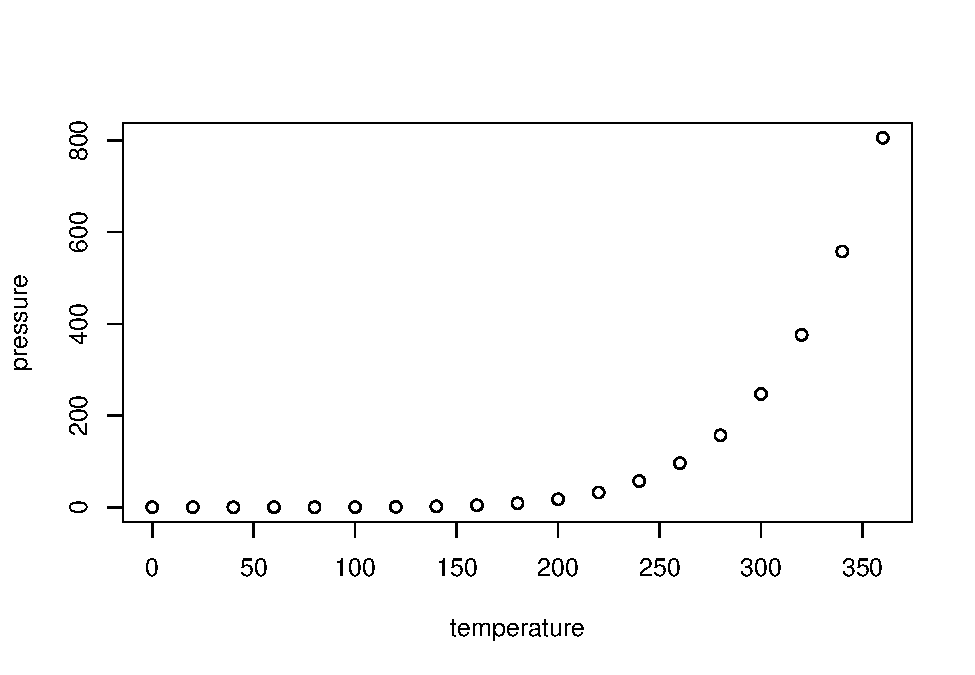
\includegraphics{1_REPORT_files/figure-latex/pressure-1.pdf}

\hypertarget{appearance-using-the-yaml-header}{%
\section{\texorpdfstring{Appearance using the \texttt{YAML}
Header:}{Appearance using the YAML Header:}}\label{appearance-using-the-yaml-header}}

We can regulate the appearance of the document from here. There's a lot
flexibility but the learning curve is somehow steep. I'll link useful
resources to learn, but, in principle, the document is \emph{ready for
writing}.

Here the corresponding references:

\begin{itemize}
\tightlist
\item
  \href{https://bookdown.org/yihui/rmarkdown/pdf-document.html}{PDF
  output}
\item
  \href{https://pandoc.org/MANUAL.html\#templates}{Pandoc Manuals}
\item
  \href{https://bookdown.org/yihui/rmarkdown/pdf-document.html\#table-of-contents-1}{TOC}
\item
  \href{https://github.com/jgm/pandoc-citeproc/blob/master/man/pandoc-citeproc.1.md}{Cite
  with Pandoc}
\end{itemize}

Here those inputs that are easy to configuration for you guys to get an
idea:

\begin{itemize}
\tightlist
\item
  With \texttt{documentclass} has three base templates:
  \texttt{article}, \texttt{report} and \texttt{book}.
\item
  \texttt{geometry} let's me change the margins.
\item
  \texttt{lof} and \texttt{lot} set to true give me a list of figures
  and tables respectively.
\end{itemize}

\hypertarget{introduction}{%
\chapter{1. Introduction:}\label{introduction}}

\begin{itemize}
\tightlist
\item
  The developement of this package takes place in the framework of the
  seminar ``Advanced Statisical Programming'' -\textgreater{} SS20
\item
  We extend the R6 class \emph{``LocationScaleRegression''} belonging to
  the \texttt{asp20model} package concieved specifficaly for this
  seminar (Riebl 2020)
\item
  Our aim is to develope an multi-faceted implementation of boosting for
  location and scale regression including component-wise boosting, use
  of cross-validation to determine the optimal stopping critera and
  useful options for visualization.
\end{itemize}

\hypertarget{description-of-progress}{%
\chapter{2. Description of progress}\label{description-of-progress}}

\begin{quote}
Hannes lead question: What are the critical aspects of your
implementation and your package? Stability? Performance?
User-friendliness? How are you going to deal with these potential
issues?
\end{quote}

Our package rely heavily on the asp20model package, any changes, or
errors in the code of the package might break the functionality.
Currently there is no validation of the given input, with respect to
heteroscedasticity.

The package also does not provide any auto optimization of the gradient
boost step-size, a wrongly picked step-size can lead to a deficient
performance, but an already implemented early stopping mechanism can
prevent an overfitting. An input check and cross-validation of the
step-size is on the to-do list. Also, the initial starting values for
Beta and Gamma can be further improved, see (Fahrmeir 2013, 219).
Further optimizations can be made to reduce the computation time, by
moving the calculation of the Projection Matrix for individual
covariates in the initialization section of the model. In regard to
User-friendliness of the package, we will try to implement further input
validation and try to write up with a comprehensive vignette containing
various examples in the next weeks.

L:

\begin{itemize}
\tightlist
\item
  user-friendliness: allow for convenient input of model, possibly as
  data.frame
\item
  stability: trying to implement automated testing (unit tests)
\item
  performance:

  \begin{itemize}
  \tightlist
  \item
    custom step size for Beta needed, otherwise slow --\textgreater{}
    improve
  \item
    move ProjectionMatrix Calculation to initializalisation to enhance
    efficiency
  \end{itemize}
\end{itemize}

\begin{quote}
\begin{enumerate}
\def\labelenumi{\arabic{enumi}.}
\setcounter{enumi}{1}
\tightlist
\item
  What design designs did you make with respect to your implementation?
  How are you going to extend the R6 class? What additional functions
  are you going to provide?
\end{enumerate}
\end{quote}

JS: During the learning process, we tried several methods to implement
the required functionality. At first, we started with a simple function
in a R-File. While looking at other online resources, we agreed on using
the asp20model packages as a requirement for our package and inheriting
the existing LocationScaleRegression class. Our
\texttt{LocationScaleRegressionBoost} R6 class implements a boosting
algorithm, two active fields within the model for calculating the best
fitting covariate with respect to Gamma and Beta and has four new
variables which are set at the initialization of the model to reduce
computation time of the Projection Matrixes during the gradient boosting
(subject to change). The package provides the gradient boost function
for the \texttt{LocationScaleRegressionBoost} class, which uses the two
model functions to optimize stepwise the Beta and Gamma Vector.

I propose a timeline where the implementation process is described step
by step as a list e.g:

\begin{enumerate}
\def\labelenumi{\arabic{enumi}.}
\tightlist
\item
  Primitive implementation of boosting
\item
  Simple boosting for location implemented
\item
  Adressed the estimation for the variance of gamma.
\item
  Johannes finished everything \#lol. 27.05.
\end{enumerate}

\hypertarget{johannes-is-gzus-2.}{%
\section{\texorpdfstring{Johannes is \emph{gzus}
\^{}\{2\}.}{Johannes is gzus \^{}\{2\}.}}\label{johannes-is-gzus-2.}}

L: implementation designs r6-Class ``LocScRegBoost''

\begin{itemize}
\tightlist
\item
  moved calculation of central calculation matrices in boosting
  algorithm to initializer of R6-Class via super-command
\item
  component-selection implemented inside R6-Class via additional
  active-fields

  \begin{itemize}
  \tightlist
  \item
    mechanism: calculation of n loss-function-values (n =
    \#gamma-parameters = \#beta-parameters), then compare to
    loss-functions of last iteration and choose highest loss-improvement
  \item
    calculation does NOT work via derivatives as Kneib suggested, but by
    Hannes' deviance-residuals
  \end{itemize}
\end{itemize}

\hypertarget{description-of-the-problem}{%
\chapter{3. Description of the
problem}\label{description-of-the-problem}}

\begin{quote}
Hannes lead question: Which open questions do you have about the
statistical model and methodology?
\end{quote}

JS : Can this model be used to mathematically evaluate outliers, for
example in the Munich rent data set -\textgreater{} use it to identify
cheap apartments

L:

\begin{itemize}
\tightlist
\item
  How does cross-validation work in order to optimize stopping?

  \begin{itemize}
  \tightlist
  \item
    This connects to other applications of boosters such as variable
    selection. Variable selection is especially viable since
    component-wise boosting is already implemented
  \end{itemize}
\item
  Is it possible to optimize the learning rate?
\end{itemize}

\hypertarget{extensions-to-be-implemented.}{%
\chapter{4. Extensions to be
implemented.}\label{extensions-to-be-implemented.}}

\begin{quote}
Hannes' Lead question: What functionality are you planning to (or did
you already) implement? What did you decide to leave out?
\end{quote}

L: Already implemented

\begin{itemize}
\tightlist
\item
  boosting for multidimensional (\textgreater2) beta and gamma
\item
  component-wise boosting
\end{itemize}

L: Ideas for further functionality

\begin{itemize}
\tightlist
\item
  better user-friendliness - allow inputs like my\_model \textless-
  gradient\_boost(formula, data = mtcars)

  \begin{itemize}
  \tightlist
  \item
    allow for model creation via dataframe-input
  \item
    this may reduce errors due to unexpected inputs
  \end{itemize}
\item
  illustrate functions of package with real dataframe (= Vignette)
\item
  Visualization of results via connecting to plot team
  \texttt{asp20plot}
\item
  functionality: predict
\item
  Include model diagnostics
\end{itemize}

JS: check when run gradientboost, if model is
LocationScaleRegressionBoost class

\hypertarget{summary}{%
\chapter{5. Summary?}\label{summary}}

\hypertarget{references}{%
\chapter*{6. References}\label{references}}
\addcontentsline{toc}{chapter}{6. References}

\hypertarget{refs}{}
\leavevmode\hypertarget{ref-R-R6}{}%
Chang, Winston. 2019. \emph{R6: Encapsulated Classes with Reference
Semantics}. \url{https://CRAN.R-project.org/package=R6}.

\leavevmode\hypertarget{ref-Fahrmeir.2013}{}%
Fahrmeir, Ludwig. 2013. \emph{Regression: Models, Methods and
Applications}. New York: Springer.

\leavevmode\hypertarget{ref-Hastie.2009}{}%
Hastie, Trevor, Robert Tibshirani, and J. H. Friedman. 2009. \emph{The
Elements of Statistical Learning: Data Mining, Inference, and Prediction
/ Trevor Hastie, Robert Tibshirani, Jerome Friedman}. 2nd ed. Springer
Series in Statistics. New York: Springer.

\leavevmode\hypertarget{ref-R-asp20model}{}%
Riebl, Hannes. 2020. \emph{Asp20model: An R6 Class for Location-Scale
Regression Models}.

\end{document}
